\section{\glsfmtlong{DSL}}
\label{sec:DSL}

The \glsfirst{DSL} is responsible for \glsfmtlong{OI} life cycle management, which includes indexing, transformation, storage, dissemination, and consumption \cite{nationalinstituteofstandardsandtechnology2016Information}.
In this section we introduce the \gls{DSL} and its fundamental components, see \Cref{fig:DSL}.

The \gls{DSL} is formed by two components (see \cref{subsec:SN} and \cref{subsec:GI}), and uses the \gls{UMS} (see \cref{subsec:UMS}) to structure the information for applications in social, search, AI and beyond.

    {
        \begin{figure}[tb!]
            \centering
            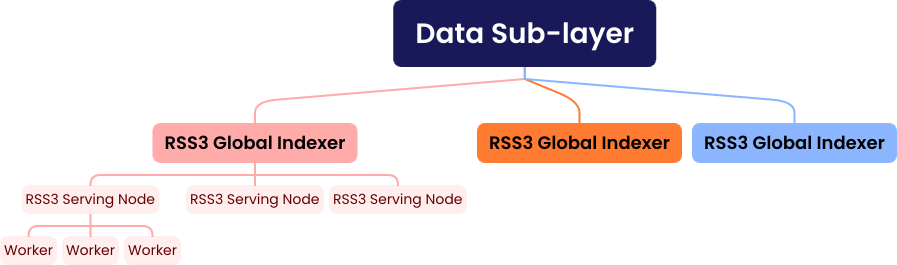
\includegraphics[width=\columnwidth]{figures/DSL.png}
            \caption{A topology of the \glsfmtlong{DSL}.}
            \label{fig:DSL}
        \end{figure}
    }


    {
        \begin{figure}[tb!]
            \centering
            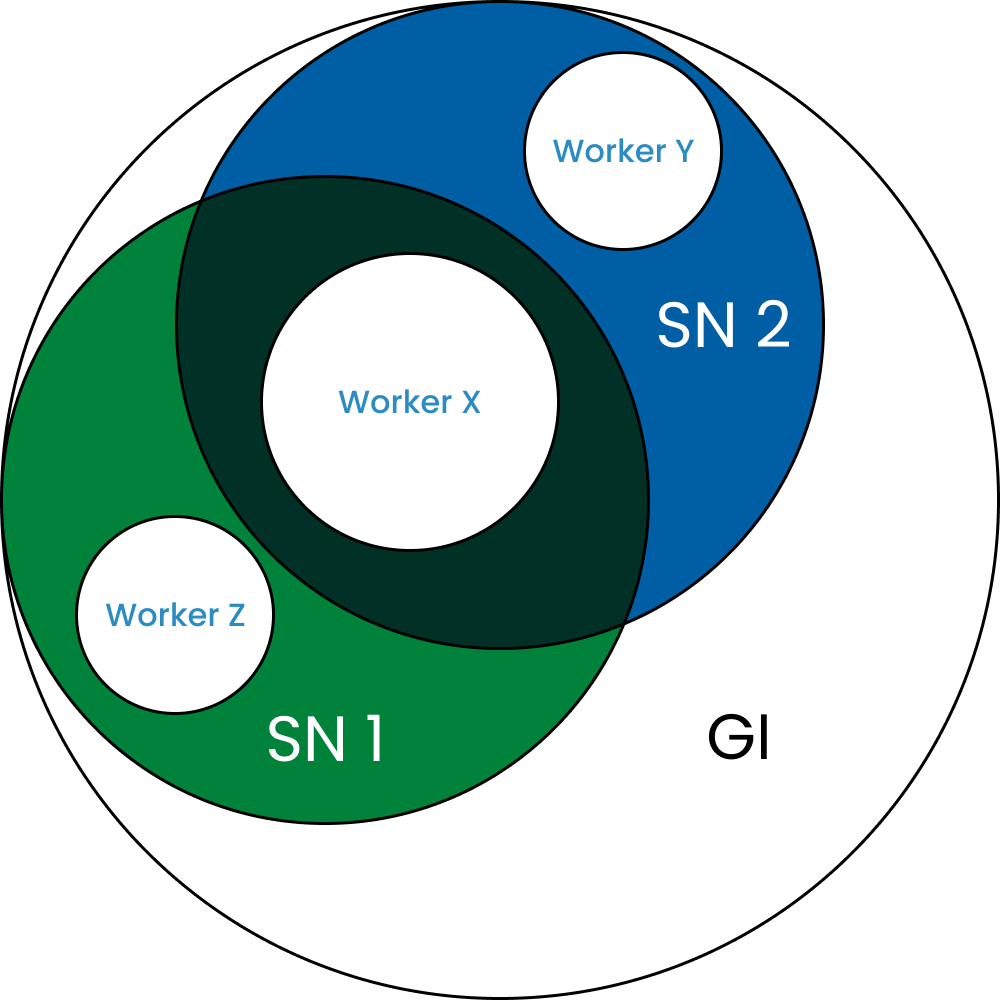
\includegraphics[width=0.7\columnwidth]{figures/GI.png}
            \caption{A venn diagram illustrating the relationship between the worker, the \glsfmtlong{SN} and the \glsfmtlong{GI}.}
            \label{fig:GI}
        \end{figure}
    }


\subsection{RSS3 \glsfmtfull{SN}}
\label{subsec:SN}

An \gls{SN}, also known as an RSS3 Node, is responsible for indexing, transforming, storing, and ultimately serving the \glsfmtlong{OI} to the end users.

The operation of an \gls{SN} is permissionless, and is subject to a set of requirements set by the Network.

\subsubsection{Indexing}
Each \gls{SN} operates a number of workers that index and structure \gls{OI} from \gls{PDS}.
Workers are community-maintained ``rules'' that define how \gls{OI} is indexed and transformed into the \gls{UMS} format.

Since each \gls{SN} is independent, it is possible for different \glspl{SN} to employ different combinations of workers to cover different \glspl{PDS}.
This design enables node operation to be flexible, accessible and affordable, in turn, offering a high degree of decentralization and robustness.

\subsubsection{Serving}
Each \gls{SN} operates a standard set of interfaces that serve structured \gls{OI} in \gls{UMS} to the end users via an \gls{GI}.

Each successful request served on the \gls{DSL} is recorded and the corresponding fees paid by the requesters are distributed to the \gls{SN}, see \Cref{subsubsec:operation_pool} for more details.

\subsection{RSS3 \glsfmtfull{GI}}
\label{subsec:GI}

A \gls{GI} is responsible for facilitating coordination among \glspl{SN} and engaging with the \gls{VSL}, and performs critical functions to ensure the \gls{DSL} is robust and reliable.

Given the importance of the \gls{GI} to the Network, its operation is not permissionless and is subject to a set of stringent requirements set by the Network.

\subsubsection{Performance Assurance} A GI acts as a load balancer and query router for end users to retrieve information from \glspl{SN}.
The unique architecture of the \gls{DSL} demands \glspl{GI} to be equipped with more computational capabilities, in order to work out the optimal route for end users to retrieve specific information from \gls{SN}, and frequently from a group of \glspl{SN} simultaneously.

\subsubsection{Quality Assurance} A GI acts as a supervisor for \glspl{SN} to ensure the quality of service.
With the \gls{DSL} being a permissionless sub-layer, the quality needs to be maintained strictly to ensure \glsfmtlong{R3N}'s robustness and reliability.
A \gls{GI} monitors the quality of \glspl{SN}, and slashes the \gls{SN} if it fails to meet the requirements.

\subsubsection{Proof-on-Chain} A GI keeps track of the work and slash records of \glspl{SN}, and submits them to the \gls{VSL} for settlement and reward allocation.

\subsection{Reliability Score} 

A \gls{GI} routes requests to \glspl{SN} based on their information coverage and a \gls{RS}.

\subsection{\glsfmtfull{UMS}}
\label{subsec:UMS}

Open Information, indexed from multiple \glspl{PDS}, is structured by \glspl{SN} into the \gls{UMS} format for interoperability.

\glspl{PDS} use different data structures, within a \gls{PDS}, there might be multiple products, services and protocols that leverage a different data structure to suit their needs.
This means limited interoperability, and developers need to look into each and every data structure, when it comes to building.
This lack of standardization means developers must investigate each unique structure individually when building applications, which is not scalable.

The \gls{UMS} addresses this issue by offering a unified set of data structures that serve as an abstraction.
This abstraction simplifies the integration process, making it more manageable and scalable for developers to work with data across various data sources.

For the complete set of the \gls{UMS}, refer to \url{https://docs.rss3.io/docs/unified-metadata-schemas}.

